%------------------------------------------------------------------------------
% Template file for the submission of papers to IUCr journals in LaTeX2e
% using the iucr document class
% Copyright 1999-2013 International Union of Crystallography
% Version 1.6 (28 March 2013)
%------------------------------------------------------------------------------

\documentclass[pdf]{iucr}              % DO NOT DELETE THIS LINE
%\documentclass[preprint]{iucr} 
\usepackage{graphicx}
\usepackage{color}
\usepackage{ulem}
\usepackage{multicol}

     %-------------------------------------------------------------------------
     % Information about journal to which submitted
     %-------------------------------------------------------------------------
     \journalcode{S}              % Indicate the journal to which submitted
                                  %   A - Acta Crystallographica Section A
                                  %   B - Acta Crystallographica Section B
                                  %   C - Acta Crystallographica Section C
                                  %   D - Acta Crystallographica Section D
                                  %   E - Acta Crystallographica Section E
                                  %   F - Acta Crystallographica Section F
                                  %   J - Journal of Applied Crystallography
                                  %   M - IUCrJ
                                  %   S - Journal of Synchrotron Radiation

\begin{document}                  % DO NOT DELETE THIS LINE

     %-------------------------------------------------------------------------
     % The introductory (header) part of the paper
     %-------------------------------------------------------------------------

     % The title of the paper. Use \shorttitle to indicate an abbreviated title
     % for use in running heads (you will need to uncomment it).

\title{TomoPy: A framework for the analysis of synchrotron tomographic data}
%\shorttitle{Short Title}

     % Authors' names and addresses. Use \cauthor for the main (contact) author.
     % Use \author for all other authors. Use \aff for authors' affiliations.
     % Use lower-case letters in square brackets to link authors to their
     % affiliations; if there is only one affiliation address, remove the [a].

\cauthor{Do\v{g}a}{G\"{u}rsoy}{dgursoy@aps.anl.gov}{} 
\author{Francesco}{De Carlo}
\author{?}{?}


\aff{Advanced Photon Source, Argonne National Laboratory, 9700 S.~Cass Ave., Argonne IL 60439-4837 \country{USA}}


     % Keywords (required for Journal of Synchrotron Radiation only)
     % Use the \keyword macro for each word or phrase, e.g. 
     % \keyword{X-ray diffraction}\keyword{muscle}

\keyword{tomopgraphy}
\keyword{x-ray imaging}
\keyword{phase retrieval}

\hyphenpenalty=10000

\maketitle                        % DO NOT DELETE THIS LINE

\begin{synopsis}
Supply a synopsis of the paper for inclusion in the Table of Contents.
\end{synopsis}

\begin{abstract}
Abstract goes here.
\end{abstract}


\section{Introduction}

Analysis of large tomographic datasets at synchrotron light sources is becoming progressively more challenging  due to the increasing data acquisition rates that new technologies in X-ray sources and detectors enable. The next generation of synchrotron facilities that are currently under design or construction throughout the world will provide diffraction limited X-ray sources and is expected to boost the current data rates by several orders of magnitude and stressing the need for the development and integration of efficient analysis tools more than ever. Several synchrotron users, to take advantage of specific instrument characteristics and specifications,  already collect data at different facilities, but they are often left alone integrating this data with the available or home-grown software tools.

There are often strong similarities within the same class of instruments that are not systematically utilized to build a coordinated software development platform or framework where each facility and user group can take advantage from or contribute in, ultimately saving on-site resources by sharing the computing tasks with the user community. Here we describe in detail an attempt to provide such a collaborative framework for the analysis of synchrotron tomographic data that has the potential to unify the effort of different facilities and beamlines performing similar tasks. The basic principles of this  Python/C++ based framework, called {\it TomoPy}, are: OS and data format independent, parallelizable, modular and supporting a functional programming style that many researchers in Academia prefer. 


\section{Background}

When it comes to the digital storage of tomographic experimental data and the development of analysis tools at synchrotron light sources around the world, the situation is very heterogeneous. As different research teams and instruments have grown at various facilities, they have often developed local data and analysis models based on instrument hardware specificity and often drawing upon the particular preferences of a scientist writing software. 

Many tomographic analysis tools utilize licensed, and often expensive, software packages like Matlab \cite{matlab} and IDL \cite{exelis_vis}, others rely on specific, and often complex to maintain, computing infrastructure like MPI-based CPU or GPU clusters. The availability of inexpensive multi-core CPU workstations and the reduced cost of computer memory  allowed to simplify the computing infrastructure required to process tomographic data \cite{rivers_spie_2012}, and started the development of single workstation tools able to perform most computing tasks. 

This transition is affecting all major synchrotron facilities where new effort is now dedicated into developing new tools that can be deployed at the facility for real time processing as well as distributed to users for off site data processing.


\section{TomoPy: A python based framework}

There is no free lunch when it comes to the integration of analysis methods. For example, Matlab's or IDL's coding practice which is based on matrix and linear algebra operations that many researchers get accustomed to come with pricy licensing fees compared to open source alternatives. R, \cite{r}, as an open-source alternative, offers a wide variety of statistical data analysis tools but has a steep learning curve and is usually hard to maintain for large projects. Python with its standard library on the other hand provides a modular, readable and manageable framework that researchers can use freely or contribute easily without facing any hassles. Besides, the native  control software running at several synchrotron facilities, EPICS, \cite{epics}, is interfaced to Python \cite{pyepics}, allowing data analysis and real-time feedback on the instrumentation status. These features make Python the method of choice for development framework.

Tomographic data processing at synchrotrons is essentially modular in nature such that the processes can be divided into a number of small independent steps. A natural way to segment the processes is to group functions according to the similarities in transformations applied on data as depicted in figure \ref{fig:ProcessSegmentation}. 


\onecolumn
\begin{figure}
\centering
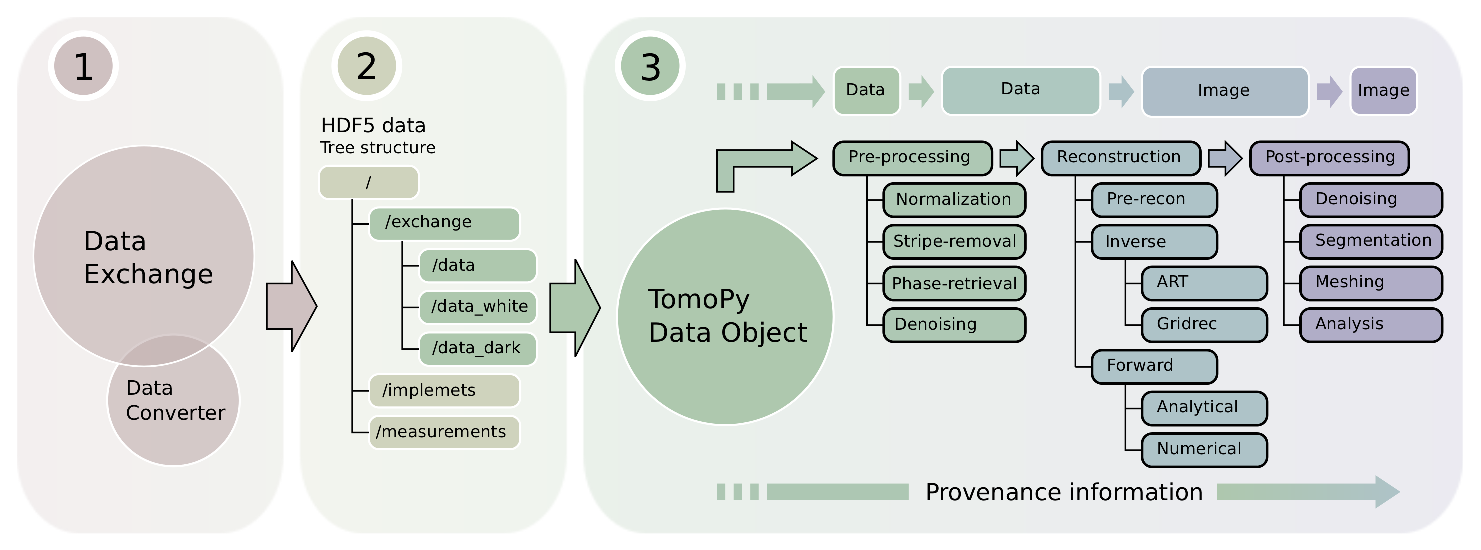
\includegraphics[width=\textwidth]{fig_framework.eps}
\caption{Processes Segmentation}
\label{fig:ProcessSegmentation}
\end{figure}
\twocolumn

{\it Explain how anyone can contribute. How it is distributed. BSD License. Documentation.}

\section{Methods} 

In synchrotron tomography, the imaging sample is placed in the beam path and the x-ray intensity profiles (also called tomograms or projections) are acquired by rotating the sample during x-ray exposure. Almost all data acquisition protocols require another set of data taken in the absence of the sample which is usually refereed to as the white-field (or flat-field) measurements. These two set of measurement together with the rotation angle information are the entry point of the analysis pipeline.

We organized tomoPy in three main categories, pre-processing, reconstruction, post-reconstruction, based on transformation types. Below are the list of function for each category currently implemented in tomoPy.

\subsection{Pre-processing module}

Preprocessing module consists of de-noising functions and aims to prepare data for the image reconstruction.

\subsubsection{Normalization}

The need for this processing step,also called flat field correction, is to compensate for the effect of optical components in the beam path which are superimposed on the projections and show up artifacts in reconstructed images. 

\subsubsection{Ring removal:}

The reconstruction quality can be dramatically degraded when local inhomogeneities consistently appear in every projection data.  This is usually caused by the impurities of the scintillation screen and non-linearity in the detector response and cannot be completely removed with the flat-field correction. These measurement artifacts usually stand out as vertical stripes in the sinograms and are transformed in the reconstructions as ring shaped artifacts. The process of clearing these artifacts is called ring-removal. 

There are numerous ways to correct these effects. The easiest and computationally most effective version is the median filtering along the sinogram. Median filtering works nicely without compromising reconstruction quality if the stripes are a few pixel width. One of the most powerful methods is the Wavelet-Fourier method \cite{Munch:09} which exploits the appearance of the ....

\subsubsection{Phase retrieval}

Single-step methods. \cite{Paganin_2002}

Touch maybe briefly multi-energy approaches with energy-selective measurements.


\subsubsection{Registration}

Data fusion: Local tomography. 

Phase-correlation: Correction of wabbling in images. Alignment for multi-step phase retrieval.

A 180 degrees rotation of the sample is generally sufficient to efficiently solve the reconstruction problem. However for some samples, especially when the sample size is larger than the field of view of the detector, a  rotation of 360 degrees can be used as an option for data acquisition. 

\subsubsection{Centering}

The quality of the image reconstruction mostly relies on an accurate determination of rotation axis position in the projections.  One common approach to determine for the center of rotation is to calculate the distance of the sinogram's center of mass from the mid-point \cite{Azevedo}. Although, this method is computationally cheaper than the alternatives, its applicability is only limited to full 360 degree datasets which makes it impractical for many situations. Another approach is to exploit the systematic artifacts in reconstructed images due to shifts in the rotation center \cite{donath_spie_2006}, see Figure~\ref{fig:OptimizeCenter2}, favorably within an optimization framework. In \textit{TomoPy} we utilize image entropy as a measure to evaluate the image quality. The corresponding cost function based on image entropy can be written as:
\begin{equation}
\arg \min_c \left\{\sum_i \sum_jH_{ij}\left[r(c)\right]\log_2 H_{ij}\left[r(c)\right]\right\}
\end{equation}
with $c$ being the unknown rotation center, $r(c)$ is the reconstructed image which is a function of $c$, and $H$ is the 2-D histogram of $r(c)$. 

The optimization problem is usually well-behaved and can be solved using any suitable optimization method in short times. For example, figure~\ref{fig:OptimizeCenter2} plots the number of iterations of the Nelder-Mead method for different initial rotation centers. The method coverges to the correct rotation center in about 20 iterations for a wide range of initial points which makes it a method of choice if robustness is desired. The problem is quite well-behaved unless one picks a very far off-center position (see figure~\ref{fig:OptimizeCenter2}). The central point of the image as an initial guess is generally more than enough for many datasets to converge to the correct rotation center in an automated fashion.

\begin{figure}
\centering
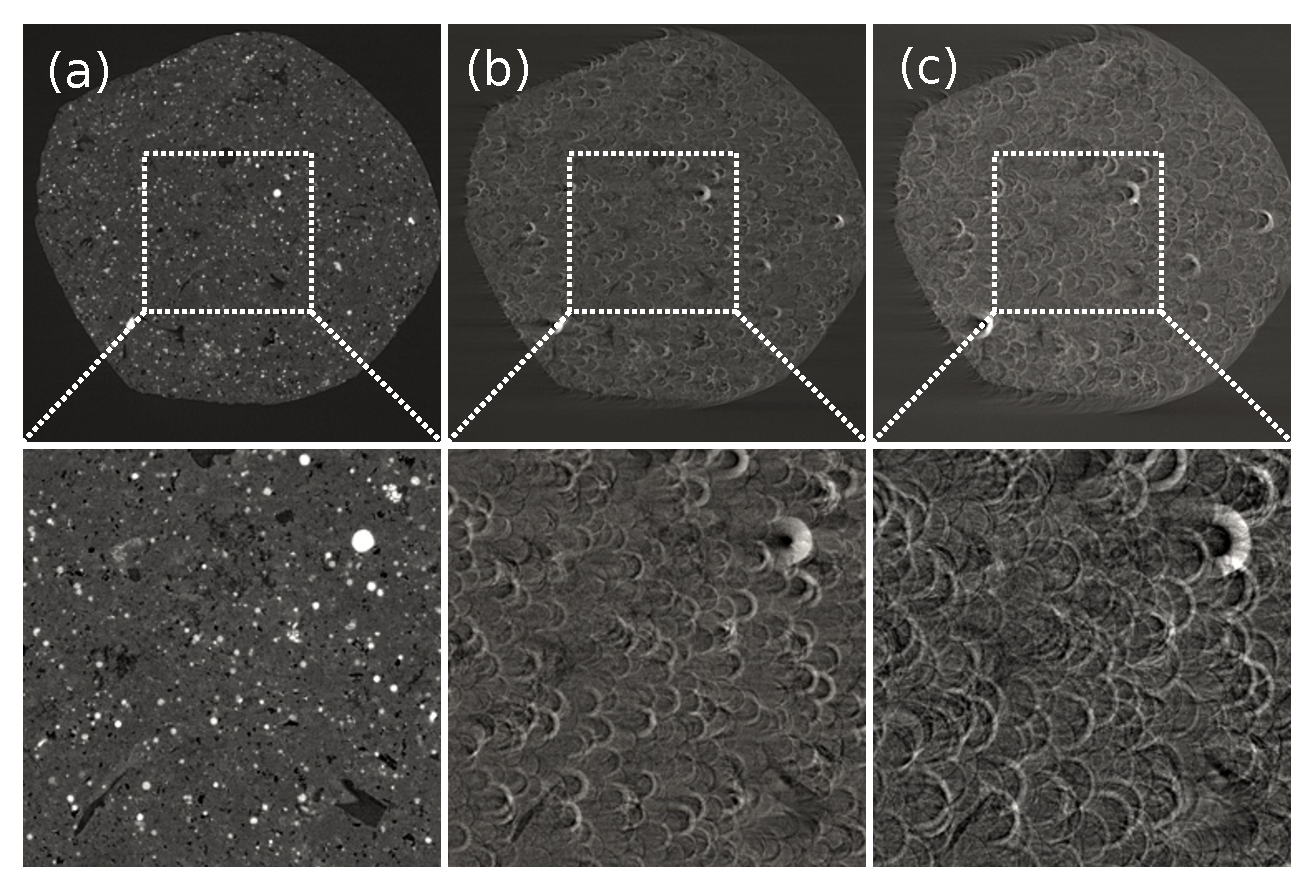
\includegraphics[width=\textwidth]{fig_center1.eps}
\caption{The images reconstructed using different centers of rotations: (a) Correct center, (b) 16 pixels  off-center horizontally, (c) 32 pixels off-center horizontally. Moving away from the correct rotation center causes image features disperse into ring shaped artifacts which in turn raises overall image entropy in the Shannon sense.}
\label{fig:OptimizeCenter1}
\end{figure}

\begin{figure}
\centering
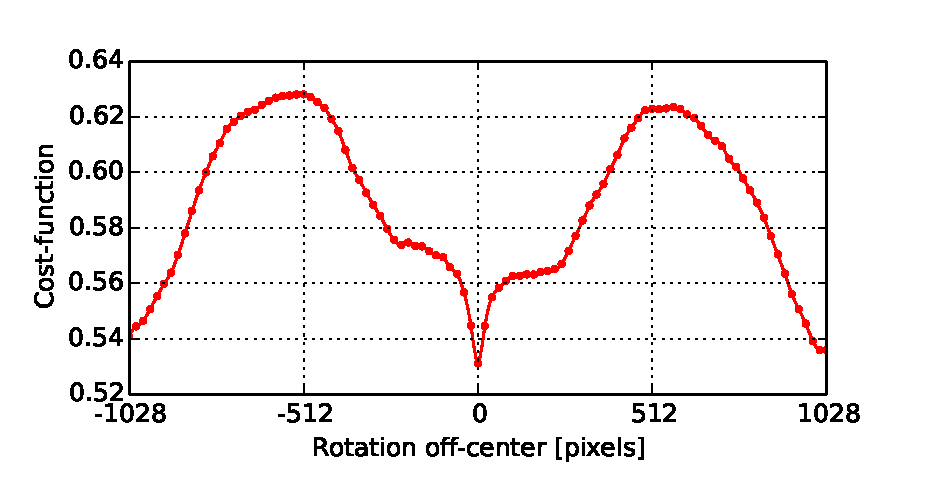
\includegraphics[width=\textwidth]{fig_center2.eps}
\caption{Error function as a function of iterations of the Nelder-Mead method for different initial rotation centers. }
\label{fig:OptimizeCenter2}
\end{figure}

\begin{figure}
\centering
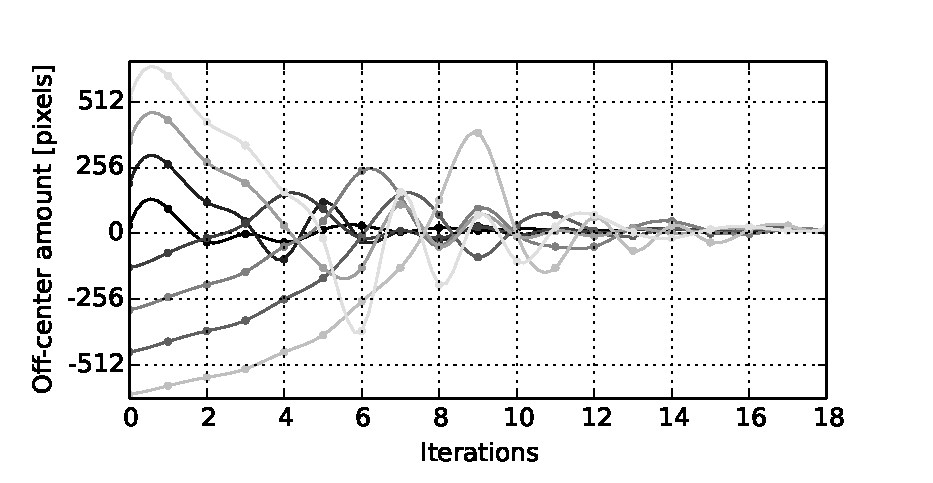
\includegraphics[width=\textwidth]{fig_center3.eps}
\caption{The image entropy as a function of rotation center in pixels.}
\label{fig:OptimizeCenter3}
\end{figure}


\subsection{Reconstruction}

\subsubsection{Gridrec}

\subsubsection{ART} 

\subsection{Post reconstruction}

??

\subsection{Storing Data}

Formats supported. Many are happy with TIFF. 

Explain storing provenance and its importance.

\section{Discussions}

Wrap the important points, vision and aims and conclude.

\appendix
\section{Appendix title}

Appendix text.

     % Acknowledgements come after the appendices

\ack{Acknowledgements}

Use of the Advanced Photon Source, an Office of Science User Facility operated for the U.S. Department of Energy (DOE) Office of Science by Argonne National Laboratory, was supported by the U.S. DOE under Contract No. DE-AC02-06CH11357

     % References are at the end of the document, between \begin{references}
     % and \end{references} tags. Each reference is in a \reference entry.

\referencelist[tomopy]

     %-------------------------------------------------------------------------
     % TABLES AND FIGURES SHOULD BE INSERTED AFTER THE MAIN BODY OF THE TEXT
     %-------------------------------------------------------------------------


 

\end{document}                    % DO NOT DELETE THIS LINE
%%%%%%%%%%%%%%%%%%%%%%%%%%%%%%%%%%%%%%%%%%%%%%%%%%%%%%%%%%%%%%%%%%%%%%%%%%%%%%

